\documentclass[a4paper]{article}

\usepackage[T5]{fontenc}
\usepackage[utf8]{inputenc}
\usepackage{amsfonts}
\usepackage{mathtools}
\usepackage[iso]{datetime}
\usepackage{tabu}
\usepackage[colorlinks=true,urlcolor=blue,linkcolor=black]{hyperref}
\usepackage{listings}
\usepackage{tikz}

\usetikzlibrary{shapes.geometric}
\tikzset{
  treenode/.style = {align=center, inner sep=0pt, text centered, font=\sffamily},
  tnode/.style = {treenode, circle, black, solid, draw=black, inner sep=2pt, minimum width=1.5em},
  subtree/.style = {draw,dashed,shape border uses incircle, isosceles triangle,shape border rotate=90, minimum height=0.5cm},
  tnull/.style = {treenode, rectangle, draw=black, minimum width=0.5em, minimum height=0.5em},
  level/.style = {sibling distance=2cm, level distance=1cm},
}

\title{Advanced Data Structures\\\large Lecture 9}
\date{2017-01-05 \\ Last edited \currenttime\ \today}
\author{Lecture by Dr. Shay Mozes\\Typeset by Steven Karas}

\newenvironment{itemize*}%
  {\begin{itemize}%
    \setlength{\itemsep}{0pt}%
    \setlength{\parsep}{0pt}%
    \setlength{\parskip}{0pt}}%
  {\end{itemize}}

\newenvironment{enumerate*}%
  {\begin{enumerate}%
    \setlength{\itemsep}{0.5pt}%
    \setlength{\parsep}{0pt}%
    \setlength{\parskip}{0pt}}%
  {\end{enumerate}}

\begin{document}

\maketitle

\section{Agenda}
Tango trees wrapup.
Link-cut trees.

\section{Tango Trees}
Built to conform to the lower bound on optimality (based on the number of changes to favored children in a static optimal tree). Tango trees are $O(\lg \lg n)$-competitive with the dynamic optimum.

As a reminder, tango trees are forests of trees of the favored paths.

\subsection{Changing the tree}\ \\
\begin{tikzpicture}
\node [subtree] (S1) {$l\quad r$}
;
\node [tnode, right of=S1, right=5cm] (S2) {$l$}
  [child anchor=north]
  child{ node [subtree] {$<l$} }
  child{ node [subtree] {$r$} }
;
\draw[->, shorten <=1cm, shorten >=1.5cm][thick] (S1) to[out=0,in=180] node [auto]{split($l$)} (S2);
\node [tnode, below of=S2, below=5cm] (S3) {$r$}
  [child anchor=north]
  child{ node [subtree] {$l<x<r$} }
  child{ node [subtree] {$>r$} }
;
\draw[->, shorten <=1.7cm, shorten >=1.7cm][thick] (S2) to[out=270,in=90] node [auto]{split($r$)} (S3);
\node [subtree, left of=S3, left=5cm] (S4) {\ }
;
\draw[->, shorten <=1.7cm, shorten >=1.7cm][thick] (S3) to[out=180,in=0] node [auto]{join($<l$, $>r$)} (S4);
\end{tikzpicture}

\section{Link-cut Trees}
Discovered by Sleator and Tarjan in 1983.
Has applications for planar graphs.
Represents trees/forests for some operations:

\subsection{Topological Operations}

\paragraph{MakeTree$(v)$}
Create a tree with a single node $v$.

\paragraph{FindRoot$(v)$}
Returns the root of the tree that contains $v$.

\paragraph{Cut$(v)$}
Assume that $v$ is not a root. Deletes the edge from $v$ to its parent.

\paragraph{Link$(v,w)$}
Given two nodes $v,w$.
Assume that $v$ is the root of its tree, and $v,w$ are not in the same tree.
Attach the tree of $v$ as a child of $w$.

\subsection{}
Weights can be assigned to either nodes or edges. Our definitions are for when the weights are defined on nodes.

\paragraph{FindMinCost$(v)$}
Find the first node with minimal cost on the path from $v$ to the root.

\paragraph{AddCost$(v, x)$}
Add $x$ to the weight of each node on the path from $v$ to the root.

\paragraph{Evert$(v)$}
Make $v$ the root of the 

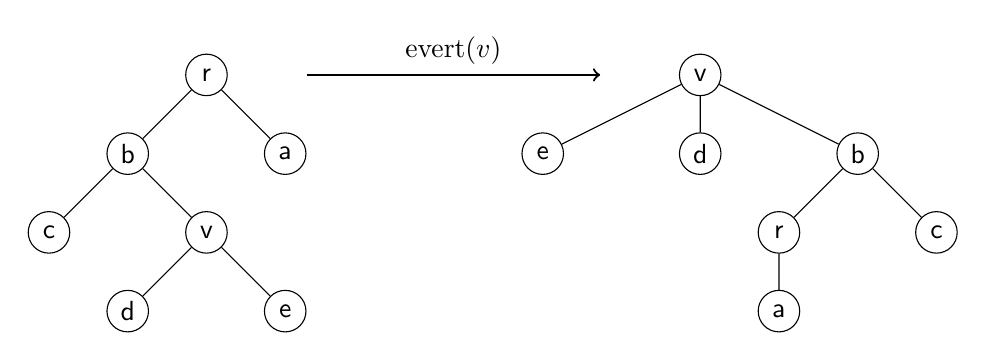
\begin{tikzpicture}
\node [tnode] (S) {r}
  child{ node [tnode] {b}
    child{ node [tnode] {c} }
    child{ node [tnode] {v}
      child{ node [tnode] {d} }
      child{ node [tnode] {e} }
    }
  }
  child{ node [tnode] {a} }
;
\node [tnode, right of=S, right=5cm] (P) {v}
  child{ node [tnode] {e} }
  child{ node [tnode] {d} }
  child{ node [tnode] {b}
    child{ node [tnode] {r}
      child{ node [tnode] {a} }
    }
    child{ node [tnode] {c} }
  }
;
\draw[->, shorten <=1cm, shorten >=1cm][thick] (S) to[out=0,in=180] node [auto]{evert$(v)$} (P);
\end{tikzpicture}

\paragraph{Complexity}
Amortized $O(\log n)$ time. Useful for planar graphs.

\subsection{Implementation}
We represent each of the trees in the forest as a forest of splay trees. 

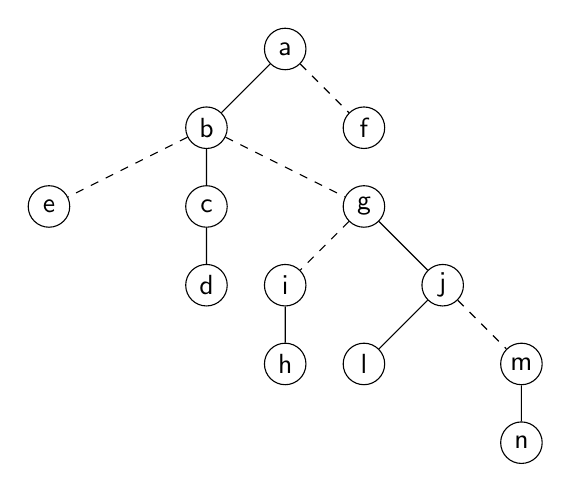
\begin{tikzpicture}
\node [tnode] (P) {a}
  child{ node [tnode] {b}
    child[dashed]{ node [tnode] {e} }
    child{ node [tnode] {c}
      child{ node [tnode] {d} }
    }
    child[dashed]{ node [tnode] {g}
      child[dashed]{ node [tnode] {i}
        child[solid]{ node [tnode] {h} }
      }
      child[solid]{ node [tnode] {j}
        % NOTE: k was deleted from the board because we didn't use it
        child[solid]{ node [tnode] {l} }
        child[dashed]{ node [tnode] {m}
          child[solid]{ node [tnode] {n} }
        }
      }
    }
  }
  child[dashed]{ node [tnode] {f} }
;
\end{tikzpicture}

%PERSONAL: I personally missed the explanation of what defines the order in the splay trees
This gives us the concrete forest of splay trees:

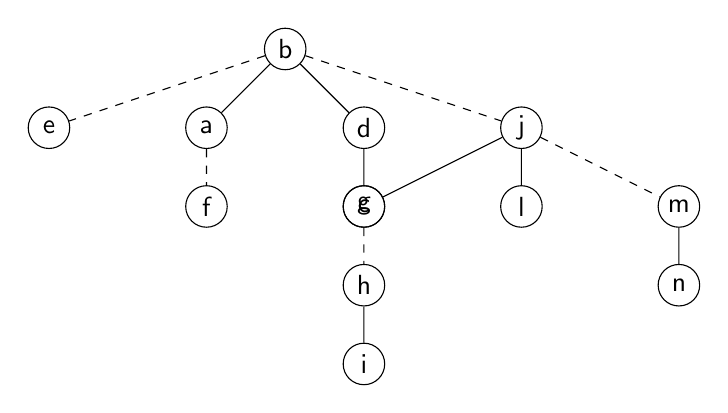
\begin{tikzpicture}
%TODO: figure out how to draw the surrounding subtrees
%TODO: figure out how to fix the overlapping nodes
\node [tnode] (P) {b}
  child[dashed]{ node [tnode] {e}}
  child[solid]{ node [tnode] {a}
    child[dashed]{ node [tnode] {f} }
  }
  child[solid]{ node [tnode] {d}
    child[solid]{ node [tnode] {c}}
  }
  child[dashed]{ node [tnode] {j}
    child[solid]{ node [tnode] {g}
      child[dashed]{ node [tnode] {h}
        child[solid]{ node [tnode] {i}}
      }
    }
    child[solid]{ node [tnode] {l}}
    child[dashed]{ node [tnode] {m}
      child[solid]{ node [tnode] {n}}
    }
  }
;
\end{tikzpicture}

The nodes of the concrete tree are the nodes of the represented tree.
Each node in the concrete tree keeps a pointer to its parent in the splay tree.
The root of each splay tree keeps a pointer to the node from which the path the splay tree represents came from (the parent of the path in the represented tree).
Each node tracks its leftmost and rightmost child in the splay tree.

\paragraph{Expose$(v)$}
This is the difficult primitive that will help us implement all the other operations efficiently. This operation makes the path from $v$ to the root a favored path and marking all favored edges that are incident to the path to unfavored.

\begin{lstlisting}[frame=L]
Expose(v):
  Splay(v)
  v.right = nil
  while v.parent != nil:
    w = v.parent
    Splay(w)
    w.right = v
    rotateUp(v)
\end{lstlisting}

So for our example above, after running Expose$(i)$:

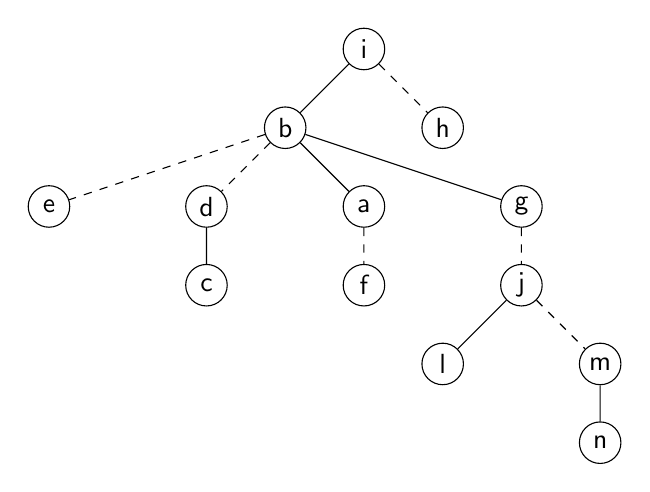
\begin{tikzpicture}
%TODO: figure out how to draw the surrounding subtrees
\node [tnode] (P) {i}
  child[solid]{ node [tnode] {b}
    child[dashed]{ node [tnode] {e}}
    child[dashed]{ node [tnode] {d}
      child[solid]{ node [tnode] {c}}
    }
    child[solid]{ node [tnode] {a}
      child[dashed]{ node [tnode] {f} }
    }
    child[solid]{ node [tnode] {g}
      child[dashed]{ node [tnode] {j}
        child[solid]{ node [tnode] {l}}
        child[dashed]{ node [tnode] {m}
          child[solid]{ node [tnode] {n}}
        }
      }
    }
  }
  child[dashed]{ node [tnode] {h}}
;
\end{tikzpicture}

After running Expose$(v)$, $v$ is the root of the splay tree that represents the favored path from $v$ to the root of the represented tree. In other words, $v$ is the root of the splay forest.

Another property after is that $v$ will have no right child.

\paragraph{FindRoot$(v)$}
\begin{lstlisting}[frame=L]
FindRoot(v):
  Expose(v)
  r = min element in splay tree of v
  Splay(r)
  return r
\end{lstlisting}

\paragraph{Cut$(v)$}
\begin{lstlisting}[frame=L]
Cut(v):
  Expose(v)
  w = v.left
  w.parent = nil
  v.left = nil
\end{lstlisting}

\paragraph{Link$(v,w)$}
\begin{lstlisting}[frame=L]
Link(v, w):
  Expose(v)
  Expose(w)
  w.right = v
  v.parent = w
\end{lstlisting}

\subsection{Analysis}
We want to show that this implementation is $O(\log n)$ amortized. Notably, we'll only prove this for Expose, since we take a constant number per other operation, and Splay has already been proven to be $O(\log n)$ amortized.

\paragraph{Expose}
$\underbrace{O(\log n)}_{\text{Splay}} \cdot \underbrace{\text{\# changes of favored children}}_{\text{\# iterations of the loop}}$

\paragraph{Lemma}
The number of changes of favored children in a sequence of $m$ operations is $O(n + m \log n)$

\subparagraph{Proof}
We will use a "heavy-light decomposition"\footnote{This may have been the first use of this decomposition, but it is widely used for data structure analysis}.
Let $size(v)$ be the number of nodes in the subtree of $v$ in the represented tree.
The edge $(v, v.parent)$ is "heavy" if $size(v) > \frac{1}{2} size(v.parent)$.
For each node, there is at most one heavy child.
For any path from the root to any node, there is at most $\log n$ "light" edges.
This is because each time we go down a "light" branch, the subtree is at least half as small.
Each edge may be either favored/unfavored, and light/heavy.
Each time a favored branch becomes unfavored, an unfavored branch must become favored.
It's enough to count the amount of branches that become favored.
In fact, we'll actually count: $L$ - the light branches that become favored; $H$ - the heavy branches that become favored.

Trivially, we can bound the light branches by $|L| \le m \cdot \log n$.
% TODO: review the video to understand why this is trivial.

In a tree, it holds that there are at most $n$ favored branches.

If a branch $e$ becomes favored more than $i$ times as part of the sequence of operations, it must have become unfavored at least $i-1$ times.\footnote{Alternative explanation: From within the heavy branches, all branches except maybe for $n$ branches become unfavored before the end of the operation sequence.}

Therefore, we can say that $|H| \le n + \text{heavy branches that become unfavored}$.

Each time a heavy branch becomes unfavored, a light branch becomes favored.
This happens at most $\log n$ times in each Expose. This gives us $|H| \le n + m\log n$.

Therefore, the number of changes is $|L| + |H| = O(n + m \log n)$.

\paragraph{}
We have shown a bound of $O((n+m\log n) \log n)$ on a sequence of $m$ operations.

In a sequence of $m$ 
$O(m \log^2 n)= O((n+(m-n)\log n)\log n)$.

\end{document}
